\section*{Phần 10.5}
\subsection*{Bài 2, 6}
Kiểm tra xem đồ thị đã cho có chu trình Euler hay không và tìm một cái nếu có. Nếu không có hãy kiểm tra xem có đường đi Euler không, nếu có hãy tìm một cái.
\begin{minipage}{7cm}
	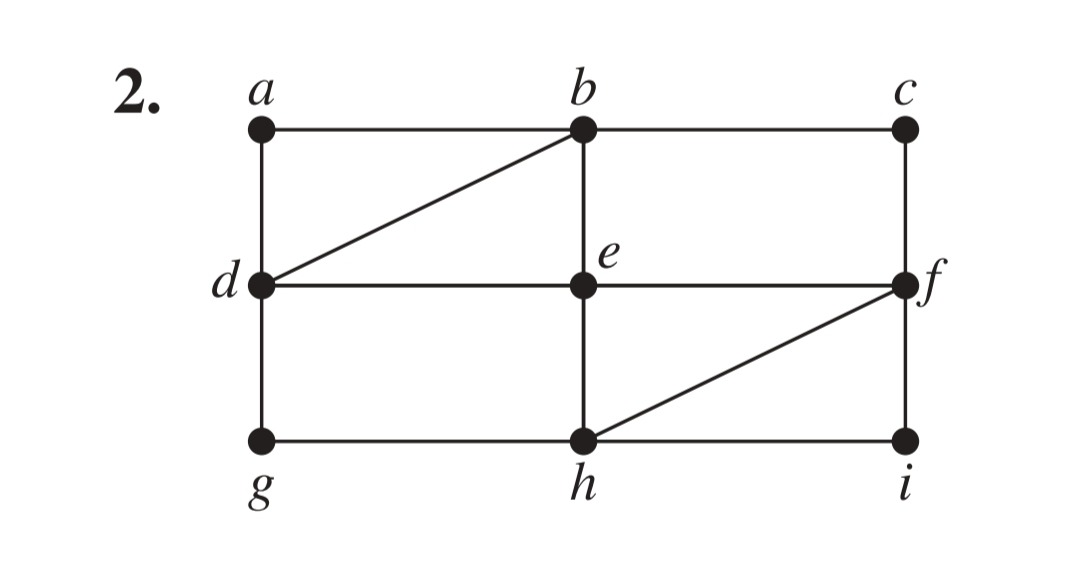
\includegraphics[scale=0.15]{10.5_2}
\end{minipage}
\begin{minipage}{7cm}
	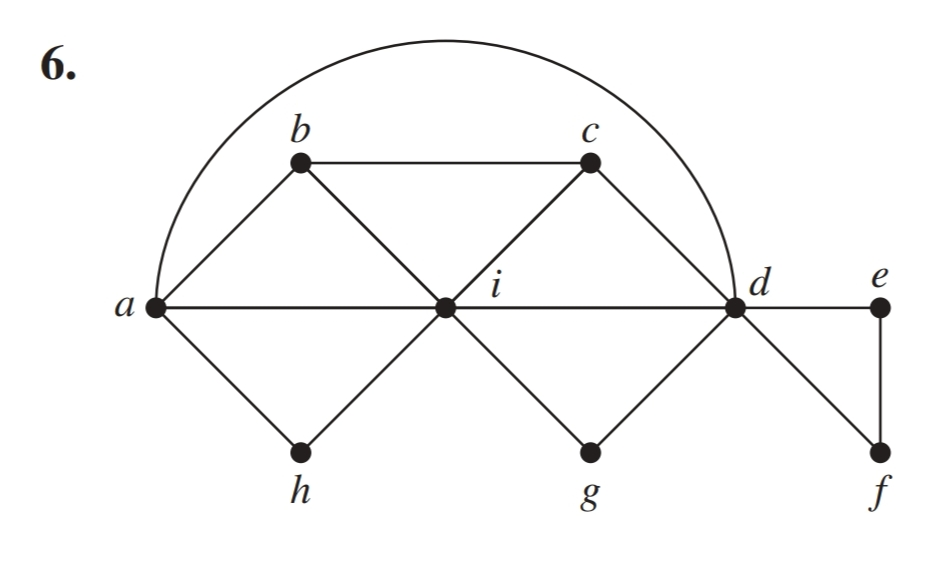
\includegraphics[scale=0.15]{10.5_6}
\end{minipage}
\begin{proof}.
	\begin{enumerate}
		\setcounter{enumi}{1}
		\item Đồ thị có chu trình Euler vì tất cả các đỉnh đều có bậc chẵn (đỉnh a, g, i, c bậc 2, còn lại bậc 4). Một chu trình Euler có thể là a, b, d, f, g, h, i, c, b, g, h, f, d, a.
		\setcounter{enumi}{5}
		\item Đồ thị này không có chu trình Euler vì có 3 đỉnh bậc lẻ (b, c bậc 3, d bậc 5) và cũng không có đường đi Euler vì nó có 3 đỉnh bậc lẻ, khi chỉ có 2 trường hợp tồn tại là không có hoặc có 2 đỉnh bậc lẻ.
	\end{enumerate}
\end{proof}
\subsection*{Bài 9}
Giả sử trong bài toán bảy cây cầu của thành phố Konigsberg, ta thêm 2 cây cầu, 1 nối từ B đến C và 1 nối từ B đến D. Có thể nào đi qua 9 cây cầu này và trở về điểm xuất phát không?
\begin{proof}
Để có thể qua được 9 cây cầu, mỗi cây đúng 1 lần và trở về điểm xuất phát ta cần tìm một chu trình Euler. Dễ thấy rằng khi thêm cây cầu thứ nhất, bậc của B và C đều là 4, nhưng sau khi thêm cây cầu thứ hai, bậc của B lúc này là 5, vậy có tồn tại đỉnh bậc lẻ, không thỏa điều kiện tồn tại chu trình, vì vậy không thể qua 9 cây cầu mỗi cây 1 lần và trở về đỉnh xuất phát.
\end{proof}
\section*{Bài 10}
Có thể đi qua toàn bộ các cây cầu trong bản đồ sau, mỗi cái đúng 1 lần và trở về vị trí xuất phát không?
\begin{center}
	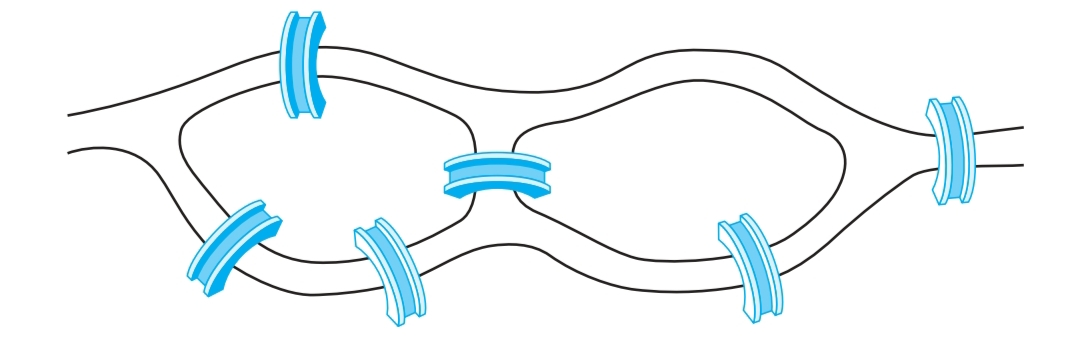
\includegraphics[scale=0.25]{10.5_10_de}
\end{center}
\begin{proof}
Ta đưa bản đồ về dạng đồ thị bằng cách chia các vùng liên thông (không thể đi qua nếu không qua cầu) được 4 vùng A, B, C, D, ta coi như 4 đỉnh.
\begin{center}
	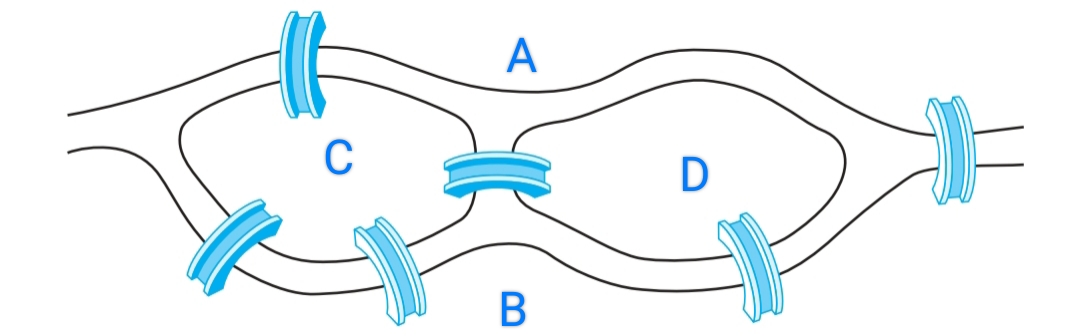
\includegraphics[scale=0.25]{10.5_10}
\end{center}
Dễ thấy rằng tất cả các đỉnh đều có bậc chẵn, vậy tồn tại một chu trình Euler, hay một đường đi qua tất cả các cây cầu và trở lại điểm xuất phát. Một đường đi có thể là A, C, B, C, D, B, A.
\end{proof}